\chapter{Signal conditioning} \label{sec:trans}

%**********************************************
\section{Voltage transducer} \label{sec:vtrans}
%**********************************************
The design chosen for the voltage peak transducer utilized a resistor divider network as well as a full wave precision rectifier, as shown in Figure \ref{fig:vtrans_circuit_diagram}. A precision rectifier is an operational amplifier circuit configuration that allows a rectifier circuit to behave like an ideal diode and rectifier, an advantage of this circuit is that it allows the rectification of voltages smaller than the forward voltage of the diode \cite{PrecisionRectifier}.
\begin{figure}[!ht]
  \centering
        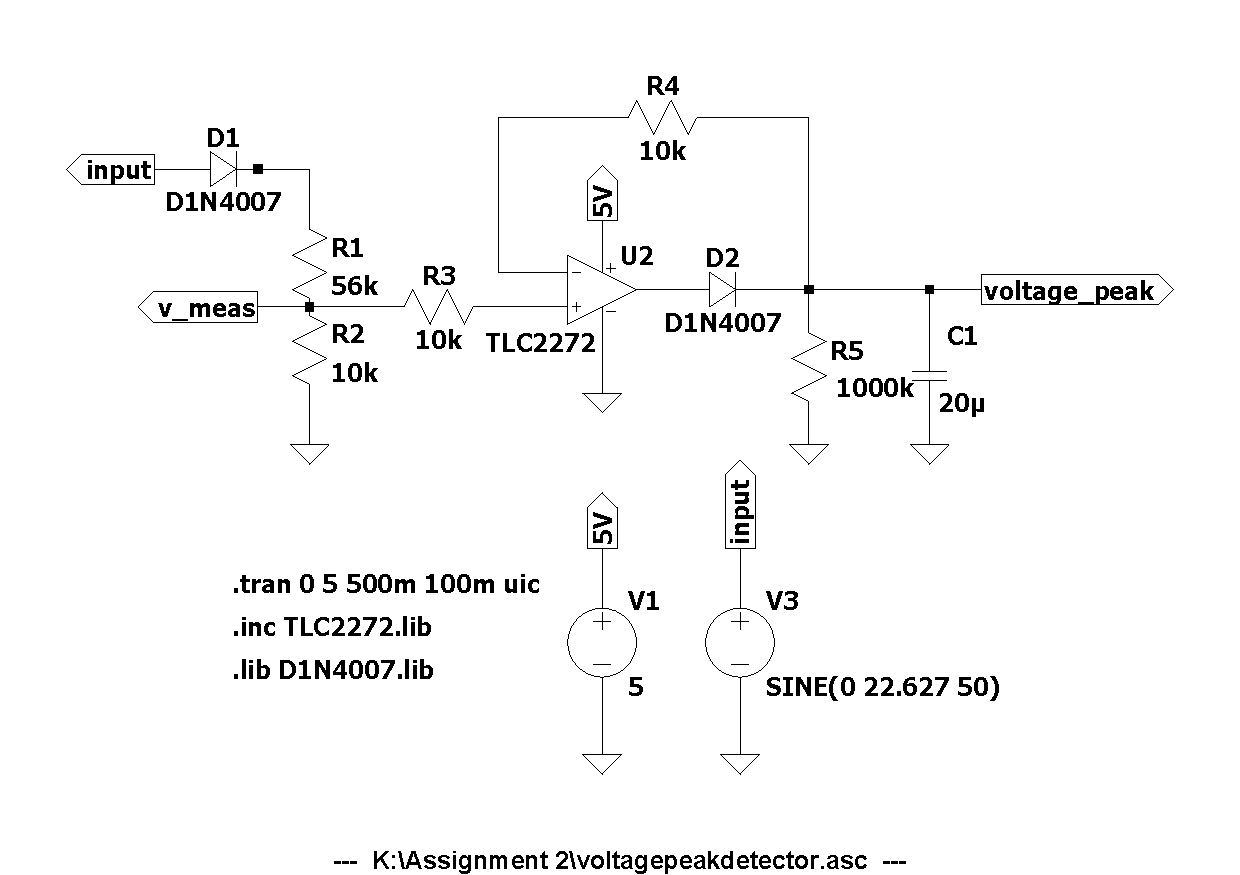
\includegraphics[width=0.5\linewidth]{./Figures/vtrans_circuit_diagram.pdf}
		    \caption{Voltage transducer circuit diagram.} \label{fig:vtrans_circuit_diagram}
\end{figure}

\subsection{Design} \label{sec:vtrans_design}
A single voltage supply configuration was used for the operational amplifier circuitry due to the \SI{-5}{V} supply rail having severe current supply limitations, as well as to keep the measurement circuitry reliable under full load conditions. It was found that the largest differential mode input to the chosen TLC2272 op amp was $V_{DD}=\SI{5}{V}$ and the absolute minimum input was found as $V_{EE}-\SI{0.3}{V}=\SI{-0.3}{V}$ \cite{TLC2272:2016}. It was also found that each TLC2272 chip required roughly \SI{2.4}{\milli A} at room temperature, given a supply voltage $V_{DD}=\SI{5}{V}$ \cite{TLC2272:2016}. An absolute maximum input voltage of \SI{24}{VAC} was chosen to ensure that the circuit could be supplied with both output voltages from the transformer. A voltage divider network was used to step this large input down to a voltage range usable by the operational amplifier for the voltage transducer circuitry.\vspace{4mm} \newline A 1N4007 rectification diode was placed in series with the voltage divider to not exceed the maximum negative differential mode input of \SI{-0.3}{V} of the TLC2272. To compensate for the forward voltage of this diode, it was found that a forward voltage of \SI{0.7}{V} could be expected when choosing a maximum current of \SI{0.4}{\milli A} through the voltage divider resistors \cite{1N4007:2014}. %Given this information the input to the resistor divider network was found to be $V_{in}=\SI{23.5}{VAC}$ and with the specified range of the Arduino being $1023$ bits, it was calculated that for this maximum input voltage the resolution of the ADC would be $\SI{8.1175}{\milli V}$ per bit. 
Given this information the input to the resistor divider network was found to be $V_{in}=\SI{23.5}{VAC}$, and by using the maximum current specification a minimum value of $\SI{10}{\kilo \Omega}$ was calculated for $R_{2}$. The value of $R_{1}$ was found by using Equation \ref{eq:voltagedivider} and rearranging the terms and substituting for the values. It was found that $R_{1}=\SI{56.6}{\kilo \Omega}$, hence a standard resistor value of $\SI{56}{\kilo \Omega}$ was chosen.
\begin{align}
   V_{DD}=\frac{R_2}{R_1+R_2}V_{in}
   \label{eq:voltagedivider}
\end{align}
Peak detection functionality was achieved by using a full wave precision rectifier as can be seen in Figure \ref{fig:vtrans_circuit_diagram} \cite{PrecisionRectifierFullwave}. To minimise any power losses in the operational amplifier, a resistor $R_3=\SI{10}{\kilo \Omega}$ was placed at its positive input pin to prevent an excess amount of current from flowing into the operational amplifier. Another resistor $R_4=\SI{10}{\kilo \Omega}$ was also placed between the non inverting input of the amplifier and the output as to ensure a minimum current flowing through to the output of the transducer during the negative half cycle of the input wave \cite{PrecisionRectifierFullwave}. 
If negative voltages are applied at the input of the precision rectifier the operational amplifier runs open loop, since the diode is reverse biased, which causes the operational amplifier to saturate. It takes time for the operational amplifier to move out of saturation, and this greatly decreases the frequency response of the circuit, thus further motivating the choice of rectifying the input voltage and supplying the operational amplifier with a single supply configuration \cite{PrecisionRectifierSaturation}. It is worth noting that the resistor $R_4$ is redundant due to the fact that the input has been rectified. \vspace{4mm} \newline
The final part of the peak detection circuit requires a capacitor and resistor with an adequate RC constant as to maintain the desired peak voltage to be measured by the Arduino. It was found that the Arduino had an extremely large analogue pin input resistance of $R=\SI{100}{M\Omega}$, and thus to simplify the design it was assumed that only the external resistor would contribute to maintaining the desired peak output voltage. A ripple voltage of no more than $\SI{5}{\milli V}$ was chosen for this design and the required capacitor could then be found by using Equation \ref{eq:ripplevoltage}. With a maximum input voltage $V_{m}=\SI{5}{V}$, a frequency of \SI{50}{Hz} and a chosen output resistor specified as $R=\SI{1}{M\Omega}$ it was found that the desired smoothing capacitor value had to be equal to $C=\SI{20}{\micro F}$ \cite{Neaman:2018}.\newline
\begin{align}
  V_{r} = \frac{V_{m}}{fRC} 
   \label{eq:ripplevoltage}
\end{align}
A design requirement of responding to a $\SI{1}{V}$ change, which corresponds to an output voltage change of $\SI{151.15}{\milli \volt}$, within 1 second was important due to the practical application of this design. Equation \ref{eq:capacitordischarge} had to be used \cite{CapacitorDischarge} in order to determine the total time taken to discharge for the chosen component values. Here $V_{s}=\SI{3.4284}{\volt}$, which corresponds to an input of \SI{16}{VAC}, and $V_{c}=\SI{3.2769}{\milli \volt}$, which corresponds to a \SI{1}{V} decrease in input peak voltage and $C=\SI{20}{\micro F}$ as calculated previously. The discharge time was found as $t=0.904s$ per volt, which successfully met the discharge time specification. 
\begin{align}
  V_{c} = V_{s}e^{\frac{-t}{RC}} \nonumber \\
  t = C(R\ln(\frac{V_{s}}{V_{c}})) \label{eq:capacitordischarge}
\end{align}
Noise on the output of this transducer had to be minimized thus two low ESR rated \SI{10}{\micro F} capacitors were placed in parallel to make an equivalent capacitance of \SI{20}{\micro F}. Decoupling capacitors were also placed at the positive voltage supply input to the TLC2272 to minimize any effects of noise from the power supply on the output of the transducer.

\subsection{Simulation} \label{sec:vtrans_simu}
The voltage transducer was simulated given a nominal input voltage of $\SI{16}{VAC}$ and the plot of this output can be seen in Figure \ref{subfig:vtrans_simu_nominput}. From this graph it can be seen that the transducer perfectly follows the input wave at steady state. The voltage transducer's response to a $\SI{1}{\volt}$ change in a $\SI{16}{VAC}$ input was simulated by using a piece wise linear voltage source to increase the input voltage by $\SI{1}{\volt}$, this output can be seen in Figure \ref{subfig:vtrans_simu_nomchange}. From this graph we can see that the voltage transducer responded to the change in input within 1 second.

\begin{figure} [!ht]
 \footnotesize
 \centering
    \begin{subfigure}[]{0.4\textwidth}
              \centering
  		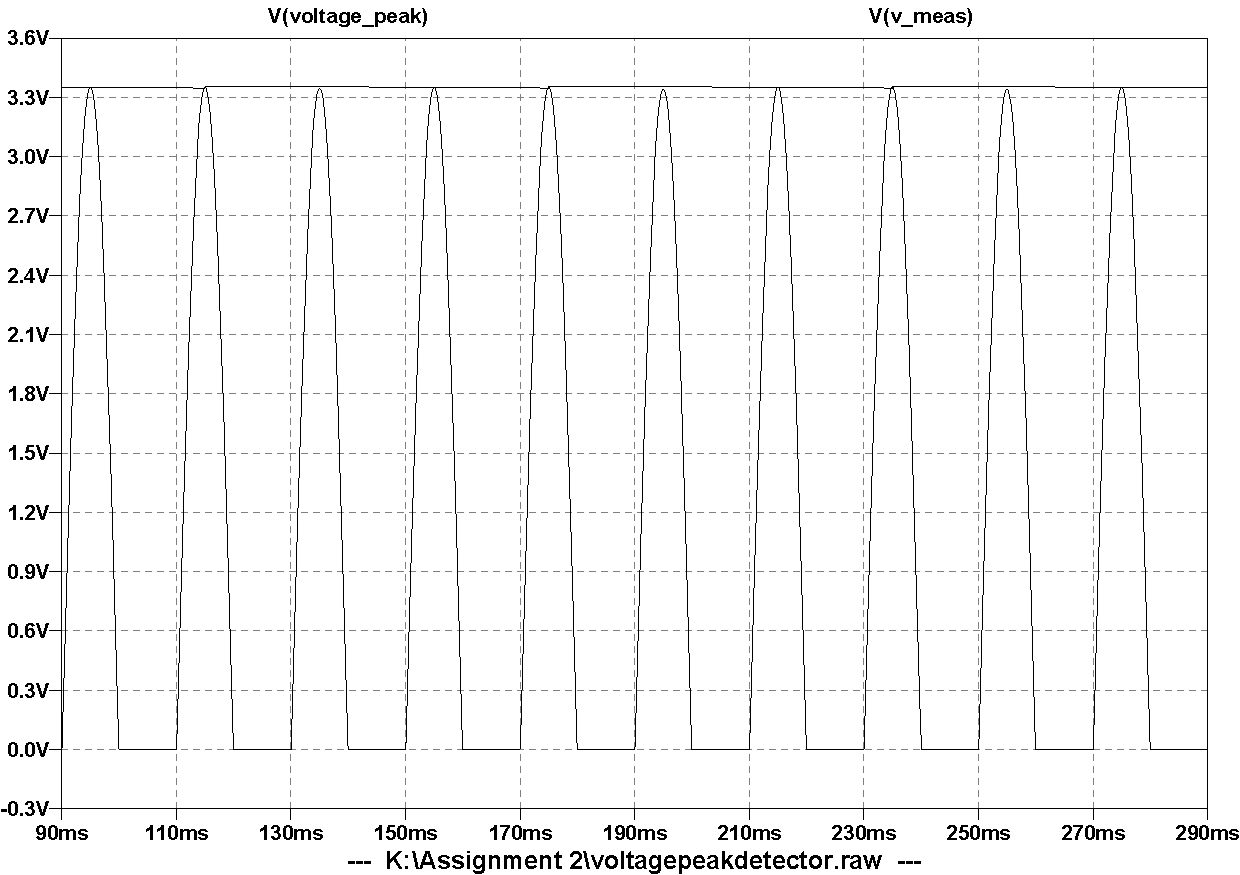
\includegraphics[width=1.0\linewidth]{./Figures/vtrans_simu_nominput.pdf}
		    \caption{} \label{subfig:vtrans_simu_nominput}
     \end{subfigure}
          \begin{subfigure}[]{0.4\textwidth}
             \centering
  		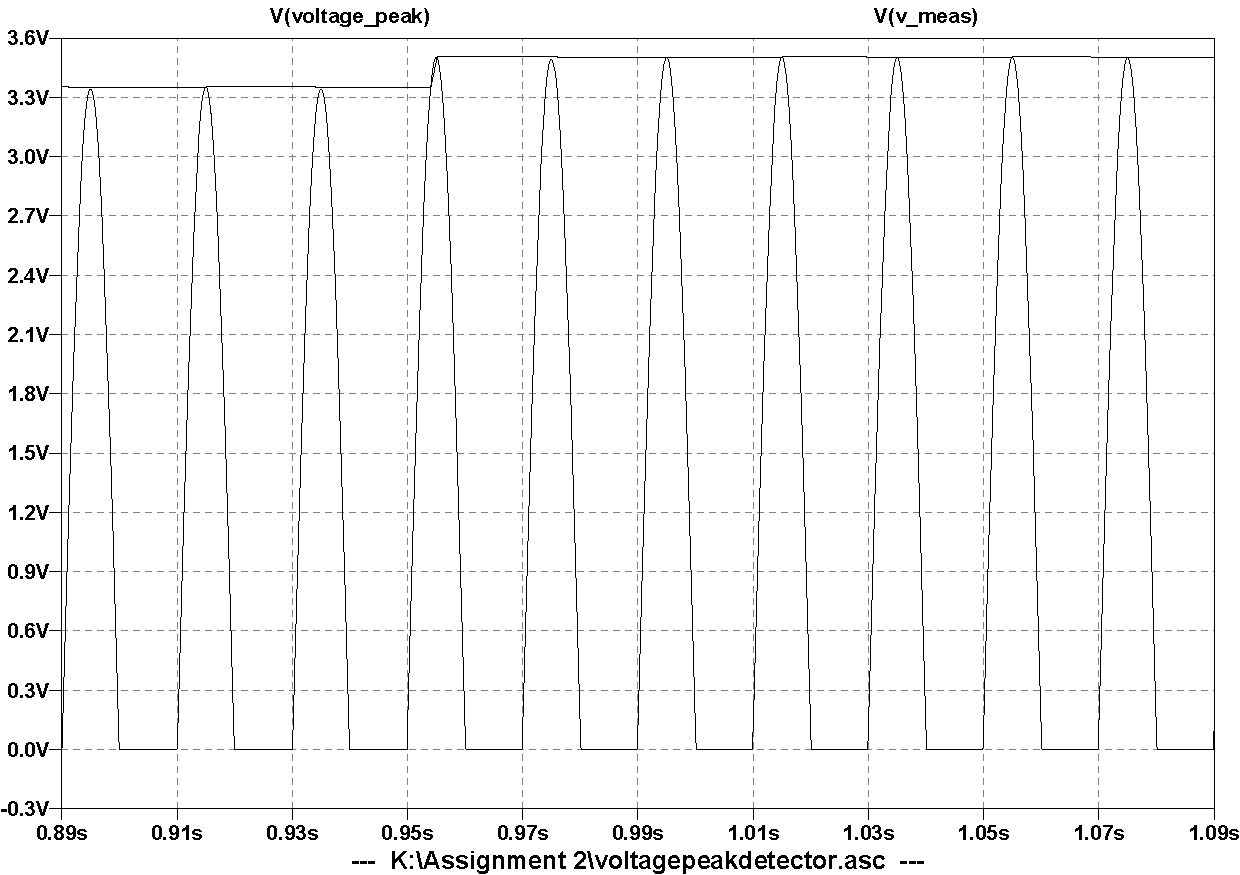
\includegraphics[width=1.0\linewidth]{./Figures/vtrans_simu_nomchange.pdf}
		   \caption{ } \label{subfig:vtrans_simu_nomchange}
     \end{subfigure}
    \begin{subfigure}[]{0.4\textwidth}
              \centering
  		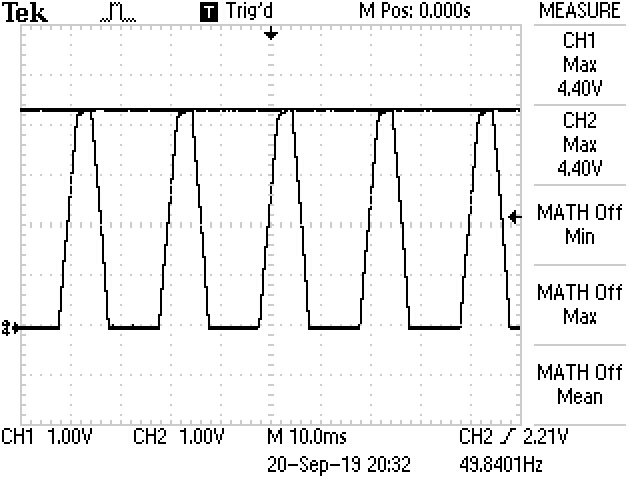
\includegraphics[width=1\linewidth]{./Figures/vtrans_meas_nom.JPG}
		    \caption{} \label{subfig:vtrans_meas_nom}
     \end{subfigure}
          \begin{subfigure}[]{0.4\textwidth}
             \centering
  		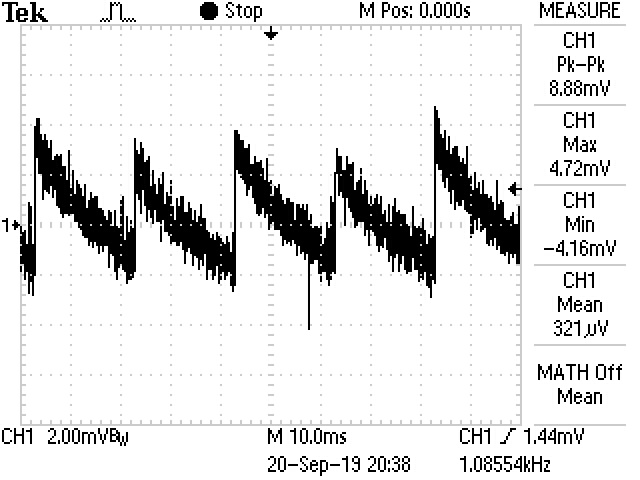
\includegraphics[width=1.0\linewidth]{./Figures/vtrans_meas_noise.JPG}
		   \caption{ } \label{subfig:vtrans_meas_noise}
     \end{subfigure}
     \caption[Voltage transducer measurement results]{Voltage transducer results. (a) Nominal load voltage simulated. (b) Response to change in input simulated. (c) Nominal load voltage measured. (d) Nominal load voltage signal quality measured.} \label{fig:vtrans_results}
\end{figure}

\subsection{Measurement} \label{sec:vtrans_meas}
Unit tests were completed using a signal generator to test various input voltages, these results can be seen in Table \ref{tab:voltagetransducerunittests}. Equation \ref{eq:pleaseworkthistimebru} was constructed from circuit analysis, and rearranged such that the applied input could be deduced given the measured ADC voltage. The applied input was deduced by Equation \ref{eq:vtransdeducedoutput} with a maximum difference of only $\SI{83.12}{\milli \volt}$ between this deduced value and the actual input voltage. Equation \ref{eq:voltagedelta} was then constructed to determine the effect of noise on the output, and a $\SI{1}{\milli \volt}$ measured ADC voltage was found to be amplified to $\SI{6.957}{\milli \volt}$. The transducer was also tested using the transformer as input under various load conditions with these results tabulated in Table \ref{tab:voltagetransducerrealtests}. Under all load conditions the deduced input differed from the actual input by no more than $\SI{118}{\milli \volt}$, confirming that the design met all requirements. The output of the voltage peak transducer, given an input from the transformer and a load of $\SI{1}{\kilo \Omega}$, can be seen in Figure \ref{subfig:vtrans_meas_nom}, with the quality of this signal shown in Figure \ref{subfig:vtrans_meas_noise}, as the $\SI{-5}{\volt}$ regulator was not used the main frequency component of the noise on the output was due to the supply voltage frequency of 50Hz. Overall it was found that the transducer could accurately detect the peak of an input voltage with a maximum output noise below $\SI{10}{\milli \volt}$.
\begin{align}
  V_{meas} = (V_{load}-V_{\gamma})\frac{R_1}{R_1+R_2} \label{eq:pleaseworkthistimebru}\\
  V_{meas} = (V_{load}-0.7)0.14374 \nonumber  \\
  V_{load} = 6.957V_{meas}+0.7 \label{eq:vtransdeducedoutput} \\
  \delta v_{load} = 6.957\delta v_{meas}\label{eq:voltagedelta}
\end{align}

%**********************************************
\section{Current transducer}\label{sec:itrans}
%**********************************************
The design for the current peak transducer consisted of a current sense resistor in series with the load, a non inverting operational amplifier gain stage, and a precision rectifier implemented as in Section \ref{sec:vtrans}, with the schematic shown in Figure \ref{fig:itrans_circuit_diagram}. A non inverting amplifier is an operational amplifier configuration where the input voltage signal is connected to the non-inverting input to the operational amplifier. The feedback control consists of a resistor divider network that connects the output to the inverting input, this resistor divider network sets the gain of the amplifier, produces a good stability and has a high input impedance \cite{NonInvertingOpAmp}.
\begin{figure}
    \centering
        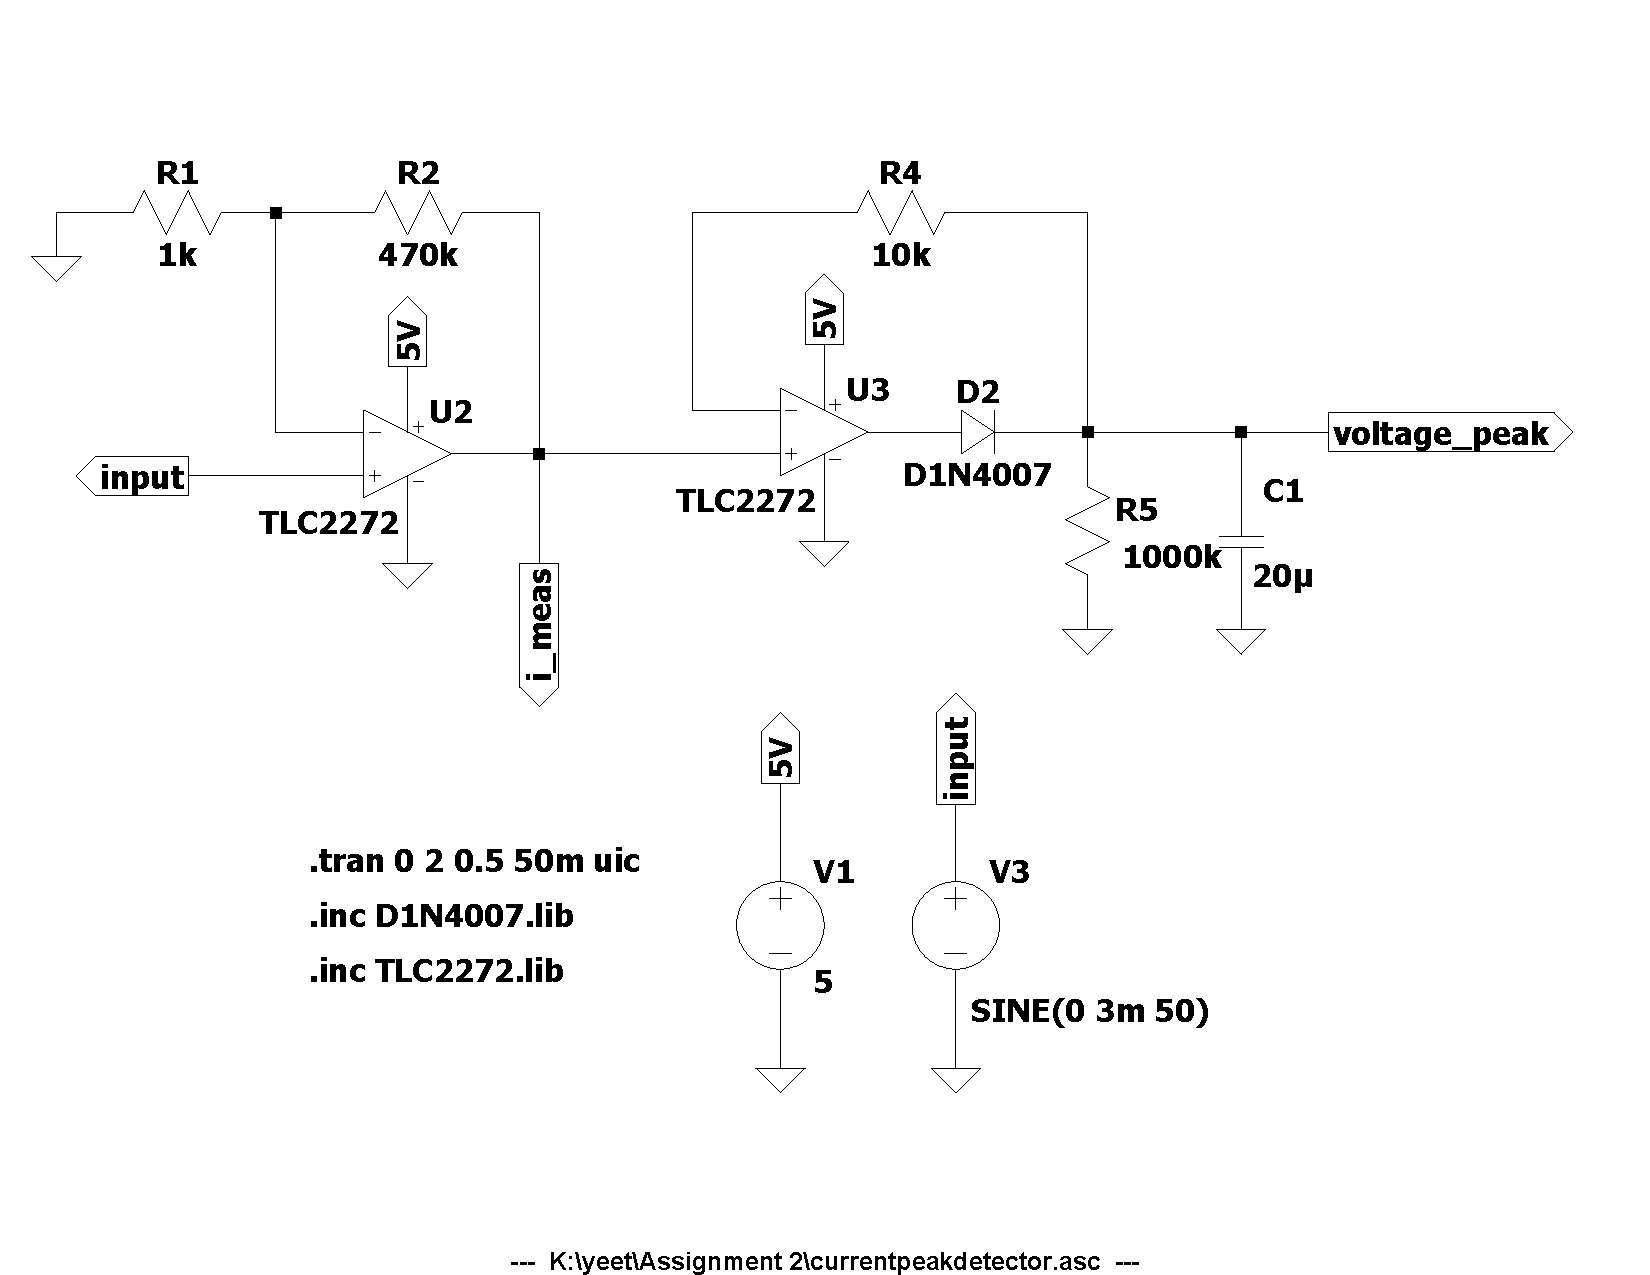
\includegraphics[width=0.5\linewidth]{./Figures/itrans_circuit_diagram.pdf}
		    \caption{Current transducer circuit diagram.} \label{fig:itrans_circuit_diagram}
\end{figure}

\subsection{Design} \label{sec:itrans_design}
A sense resistor was added in series with the load to translate a current measurement into a voltage measurement, this voltage measurement was then amplified to a suitable voltage level usable by the peak transducer. A $\SI{30}{\milli \Omega}$ sense resistor was chosen which ensured a reasonable trade off between power losses in the system and the measured voltage fain required for the amplification stage. Finally it was chosen that the current peak transducer would be able to measure a maximum current of \SI{350}{\milli A}, this corresponded to a sense voltage of \SI{10.5}{\milli V}. The Arduino's maximum pin voltage was given as \SI{5}{\volt}, and to ensure a maximum resolution for the \SI{350}{\milli A} measurement range, the \SI{10.5}{\milli V} maximum sense voltage had to be amplified using a operational amplifier. The configuration chosen for the amplification stage was a differential mode non-inverting amplifier utilizing only the \SI{5}{\volt} and rail as its power supply. It was found that the maximum input to any of the operational amplifier's pins was not to exceed \SI{5}{\volt} or \SI{-0.3}{\volt} \cite{TLC2272:2016}.
The desired gain for the intermediary stage, and corresponding ratio between $R_1$ and $R_2$ was calculated by using Equation \ref{eq:opampgain}. Here $R_1$ was chosen as $\SI{1}{\kilo \Omega}$, and given this $R_2$ was found to be $\SI{470}{\kilo \Omega}$.\newline
\begin{equation}
   \frac{V_{out}}{V_{in}}=1+\frac{R_2}{R_1} 
   \label{eq:opampgain}
\end{equation}
The same design procedure as in Section \ref{sec:vtrans_design} could be applied to measure the amplitude of the peak of the amplified sinusoidal input. However as the non-inverting operational amplifier had a high output impedance the input resistor to the precision full wave rectifier could be omitted, and as before the feedback resistor was redundant as the input to this operational amplifier had been rectified. A ripple voltage of no more than \SI{5}{\milli \volt} was chosen, and from this the output capacitor to the current transducer was calculated in exactly the same way as in Section \ref{sec:vtrans_design}. \vspace{4mm} \newline
As before the desired capacitor value was found as $\SI{20}{\micro F}$ and by the same reasoning as in Section \ref{sec:vtrans_design}, by Equation \ref{eq:capacitordischarge} and the procedure followed to determine the response time given a change in input, it can be shown that the capacitor value chosen responds to a change in input in a timely fashion. To minimise the effect of noise on the output of the transducer, two \SI{10}{\micro F} low ESR capacitors were placed in parallel and decoupling capacitors were placed at the positive rail of the TLC2272 to keep the effects of the rail voltage noise from the power supply to a minimum.
 
\subsection{Simulation} \label{sec:itrans_simu}
The designed circuit was supplied with a nominal input voltage of \SI{3}{\milli \volt}, corresponding to a \SI{100}{\milli A} current through the sense resistor, this output can be seen in Figure \ref{subfig:itrans_simu_nomload}. From the graph we can see that the output of the current peak transducer perfectly follows the amplified sinusoidal input signal at steady state, this confirms that the circuit design was implemented successfully. To ensure that the current peak transducer responded to a \SI{10}{\milli A} change in input for inputs over \SI{100}{\milli A} within 1 second, a \SI{3}{\milli \volt} input was applied and increased by \SI{300}{\micro \volt}. This change in input voltage corresponded to an increase in load current by \SI{10}{\milli A}. The result of this simulation can be seen in Figure \ref{subfig:itrans_simu_change}, and from this graph we can see that the input responded to the change in input in within 1 second. 
\begin{figure} [!ht]
 \footnotesize
 \centering
    \begin{subfigure}[]{0.4\textwidth}
              \centering
  		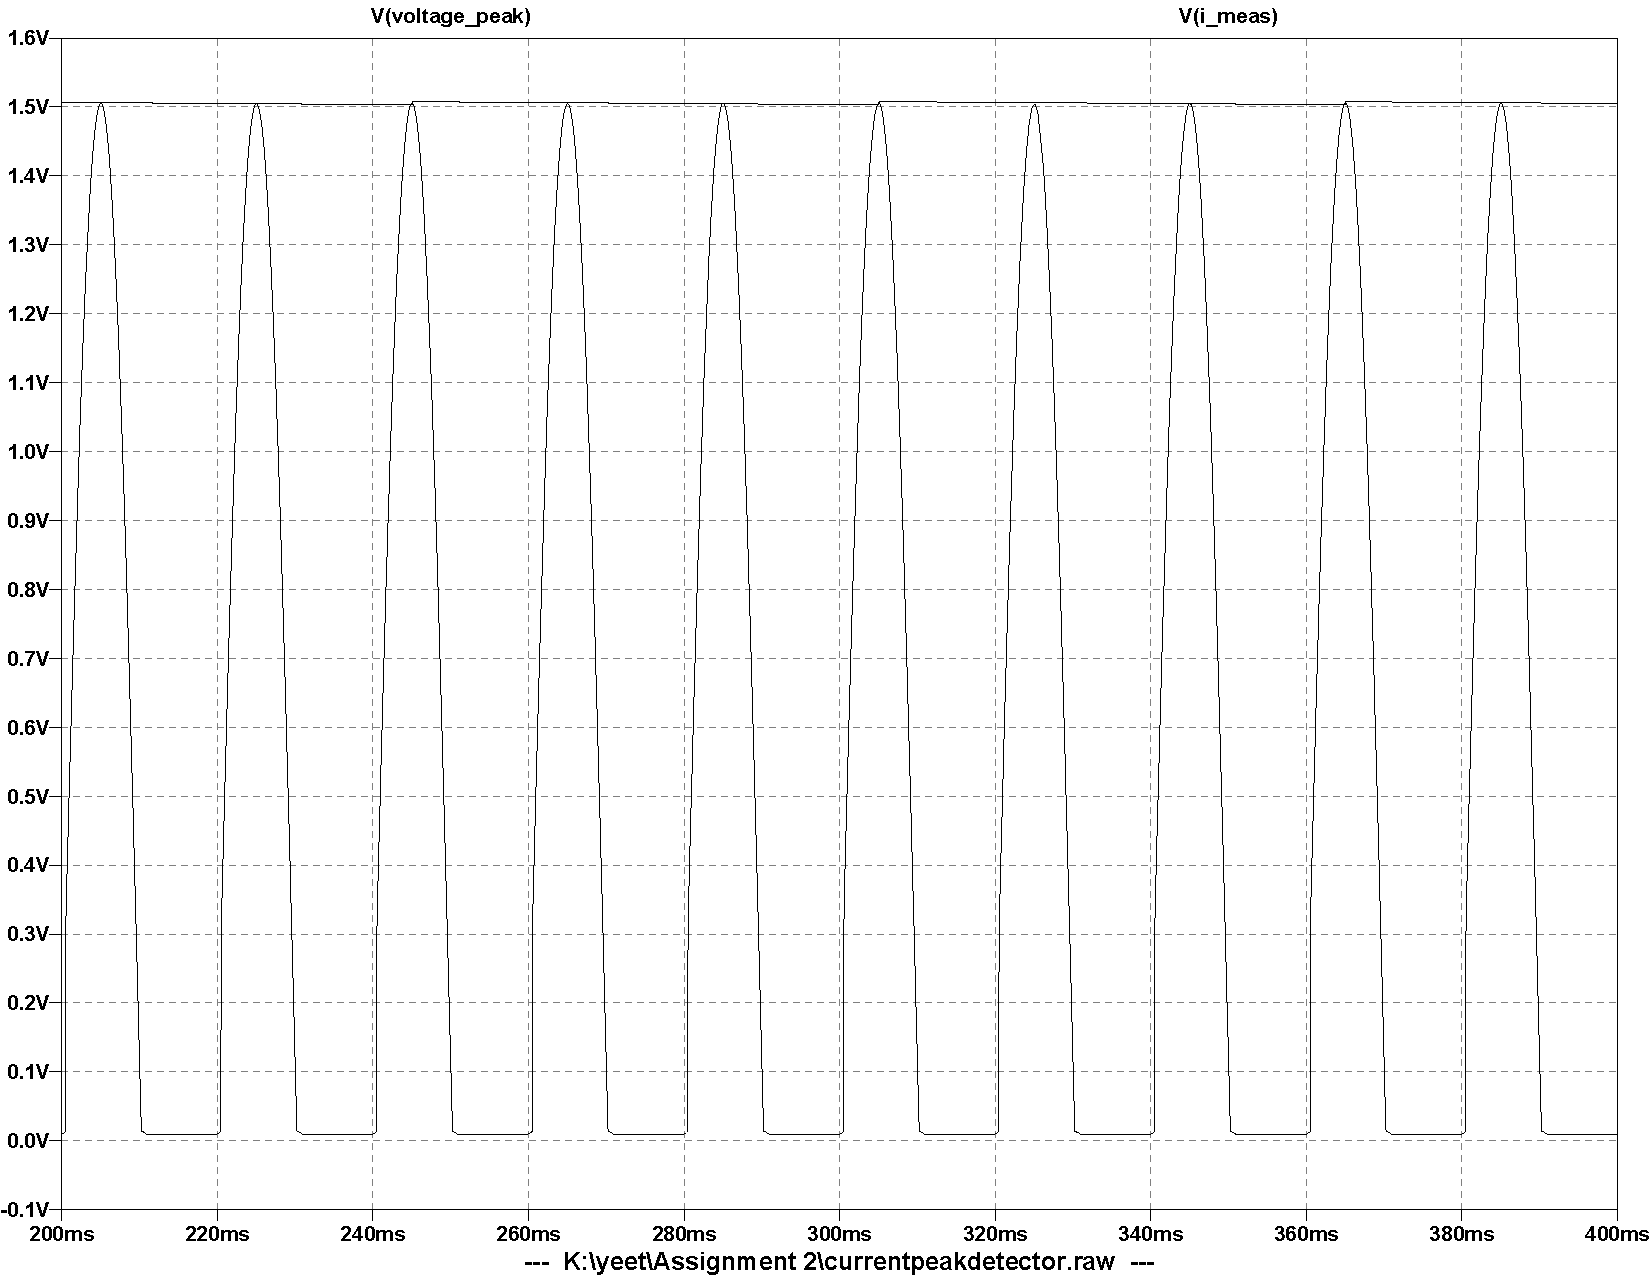
\includegraphics[width=1\linewidth]{./Figures/itrans_simu_nomload.pdf}
		    \caption{} \label{subfig:itrans_simu_nomload}
     \end{subfigure}
          \begin{subfigure}[]{0.4\textwidth}
             \centering
  		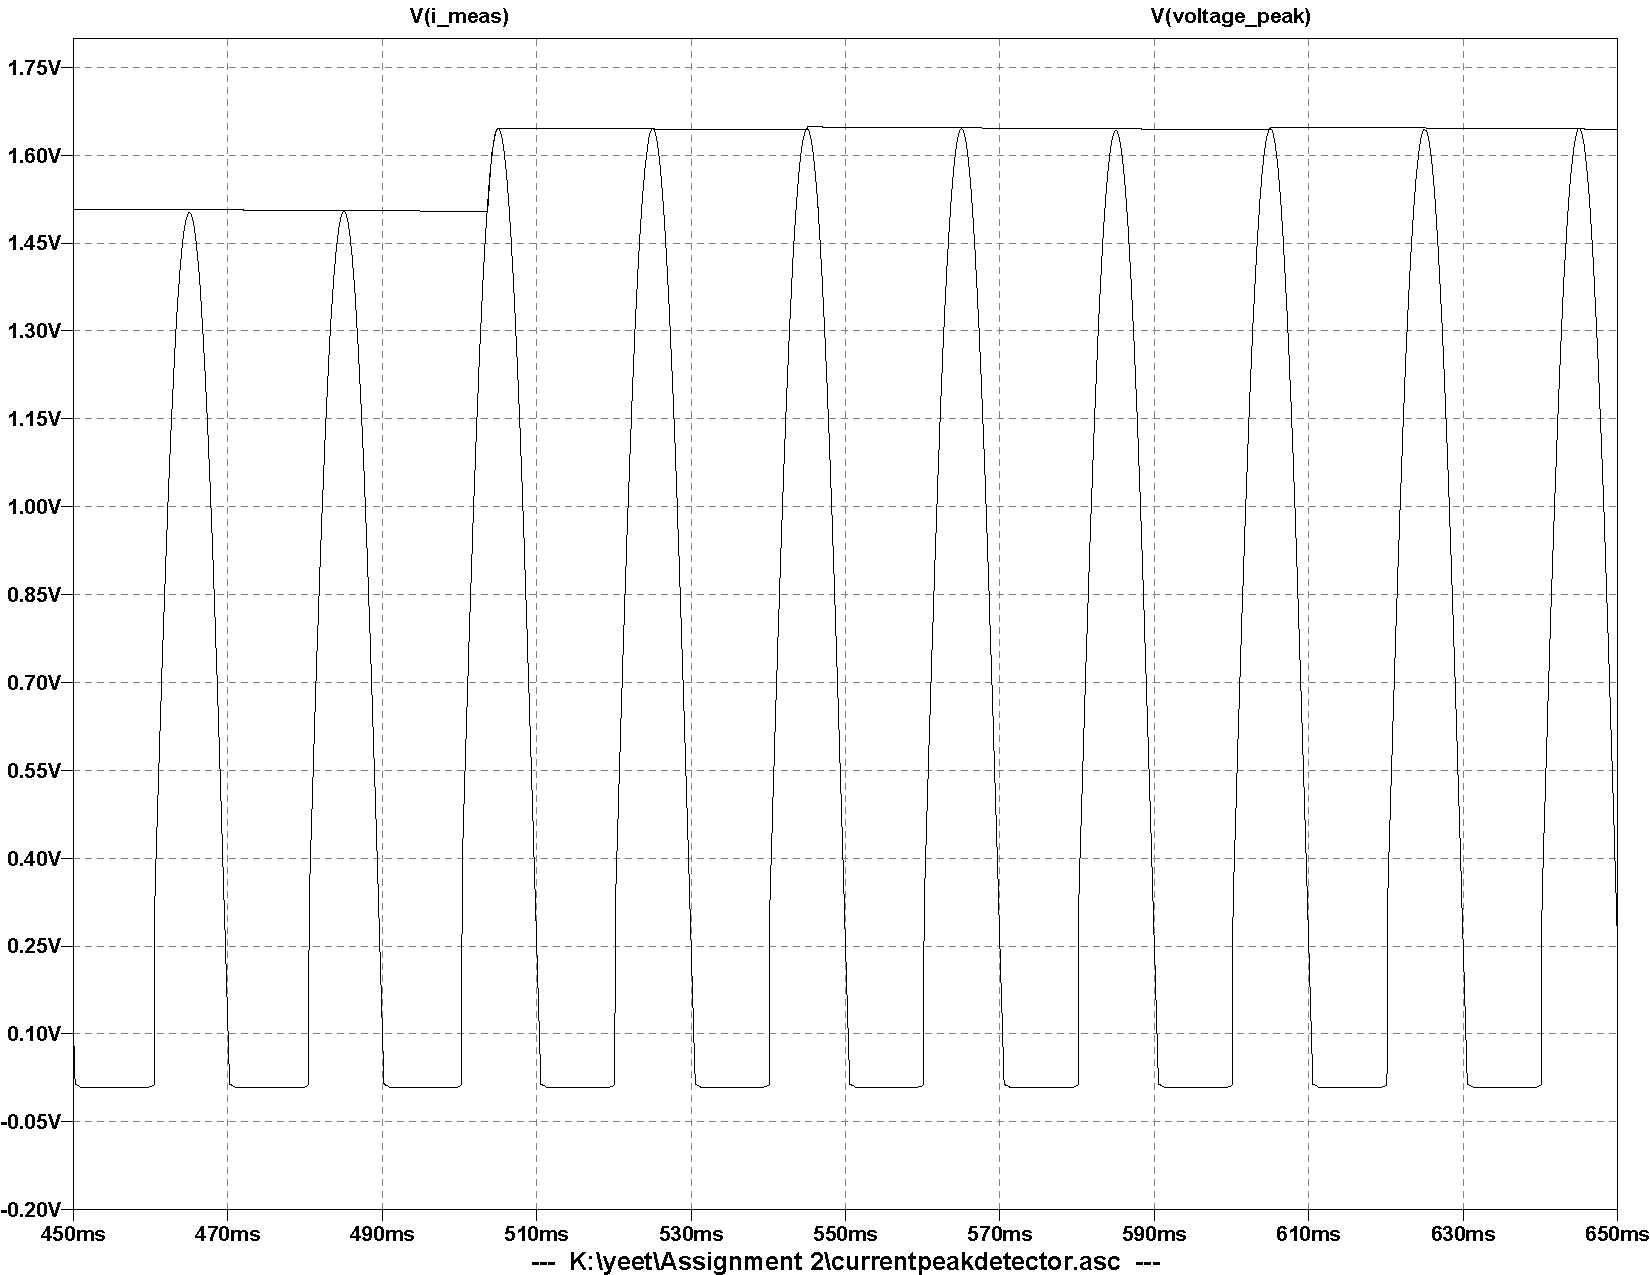
\includegraphics[width=1.0\linewidth]{./Figures/itrans_simu_change.pdf}
		   \caption{ } \label{subfig:itrans_simu_change}
     \end{subfigure}
    \begin{subfigure}[]{0.4\textwidth}
              \centering
  		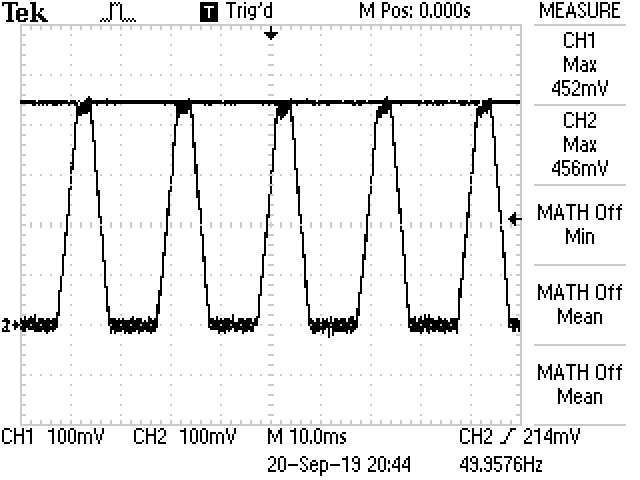
\includegraphics[width=1\linewidth]{./Figures/itrans_meas_nom.JPG}
		    \caption{} \label{subfig:itrans_meas_nom}
     \end{subfigure}
          \begin{subfigure}[]{0.4\textwidth}
             \centering
  		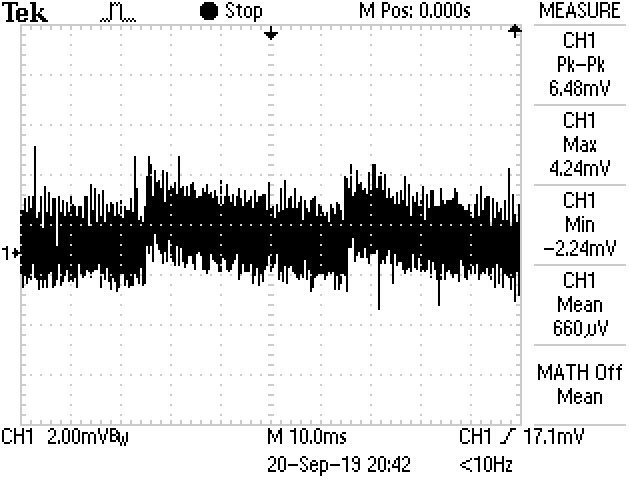
\includegraphics[width=1.0\linewidth]{./Figures/itrans_meas_noise.JPG}
		   \caption{ } \label{subfig:itrans_meas_noise}
     \end{subfigure}
     \caption[Current transducer measurement results]{Current transducer results. (a) Nominal load current simulated. (b) Response to change in load simulated. (c) Nominal load current measured. (d) Nominal load current signal quality measured.} \label{fig:itrans_results}
\end{figure}

\subsection{Measurement} \label{sec:itrans_meas}
In order to test the accuracy and precision of the current peak transducer unit tests were performed using an oscilloscope and voltage divider. Since the oscilloscope could not output the small voltages required for the unit tests a voltage divider that divided the oscilloscope output down by a factor of 100 was required in order to obtain the sense voltages in the milli-volt range. The input current was related to the output voltage by using Equation \ref{eq:currentderiv}, which was derived from circuit analysis and simplified so that the input current could be deduced given the ADC voltage as shown in Equation \ref{eq:currentcalculation}. Equation \ref{eq:currentdelta} displays the effect of noise superimposed on the input current and its effect on the measured ADC voltage, with a \SI{1}{\milli A} noise measurement being amplified to \SI{70.3}{\micro \volt}. The actual gain of the operational amplifier gain stage was calculated to be $A_{v}=474.4$ using Equation \ref{eq:opampgain}, and the resistor values for this formula were measured using a multimeter.
\begin{align}
    V_{meas}=R_{sense}I_{load}A_{v}  \label{eq:currentderiv}\\
    V_{meas}=(30m)(474.4)I_{load} \nonumber \\
    I_{load}= 0.0703V_{meas} \label{eq:currentcalculation} \\
    \delta i_{load}= 0.0703\delta v_{meas} \label{eq:currentdelta}
\end{align} 
The second column in Table \ref{tab:currenttransducerunittests} shows the output as shown on the oscilloscope screen, and the third column shows the measurement found by measuring this output using an oscilloscope. This third column was the input to the voltage circuit, with the actual sense voltage being measured as these values divided by 100. All unit tests were found to be accurate within a maximum difference of only \SI{0.74}{\milli A}, confirming that the design met the requirements. \vspace{4mm} \newline 
The current peak transducer was then tested under real measurement conditions using various load resistors, these results are tabulated in Table \ref{tab:currenttransducerrealtests}, here it was found that all measurements except the no load test was within the \SI{1}{\milli A} design specification. This contradicts the result of the no load measurement difference shown in Table \ref{tab:currenttransducerunittests}, however this difference can be explained by the fact that the input to the operational amplifier was grounded by the signal generator for the unit test, and left floating for the real no load test. \vspace{4mm} \newline  
Figure \ref{subfig:itrans_meas_nom} shows the output of the current peak transducer given a load of  $\SI{1}{\kilo \Omega}$, from the oscilloscope measurements we can see that the difference between the signals is only $\SI{4}{\milli V}$, which by using Equation \ref{eq:currentcalculation} is only out by $\SI{0.281}{\milli A}$. The signal quality of the transducer output is shown in Figure \ref{subfig:itrans_meas_noise}, which has a peak to peak range of only $\SI{15.6}{\milli V}$, this verifies that the transducer meets the specified accuracy requirements. As with the voltage peak transducer the \SI{-5}{\volt} regulator was not used for this design and thus the main frequency component of the noise superimposed on the output was due to the 50Hz frequency of the supply voltage. \vspace{4mm} \newline Due to the fact that the current peak transducer measurements were all within $\SI{1}{\milli A}$ of the actual measurement it was decided that no curve of best fit would be necessary to improve the quality of this design.

%**********************************************
\section{Phase-shift transducer}\label{sec:ptrans}
%**********************************************
The design chosen for this transducer comprises the use of voltage comparators used as zero crossing detectors, a XOR gate as well as a low pass filter, with the schematic shown in Figure \ref{fig:ptrans_circuit_diagram}. An operational amplifier comparator is a circuit that compares one analogue voltage level with a reference voltage and outputs a signal based on this voltage comparison, this operational amplifier is used in open loop mode and switches between its two saturated states \cite{OpAmpComparator}. A XOR gate is a digital logic gate with two or more inputs and one output and performs the exclusive disjunction between these input voltage levels \cite{XORGate}. A low pass filter is a circuit that allows signals with a frequency lower than that of the cut-off frequency to pass through it, and blocks all frequencies higher than the cut off frequency. A single pole low pass filter consisting of a resistor and a capacitor can be used to smooth a PWM signal into an analogue voltage level \cite{PWMref}.
\begin{figure} [!ht]
  \centering
        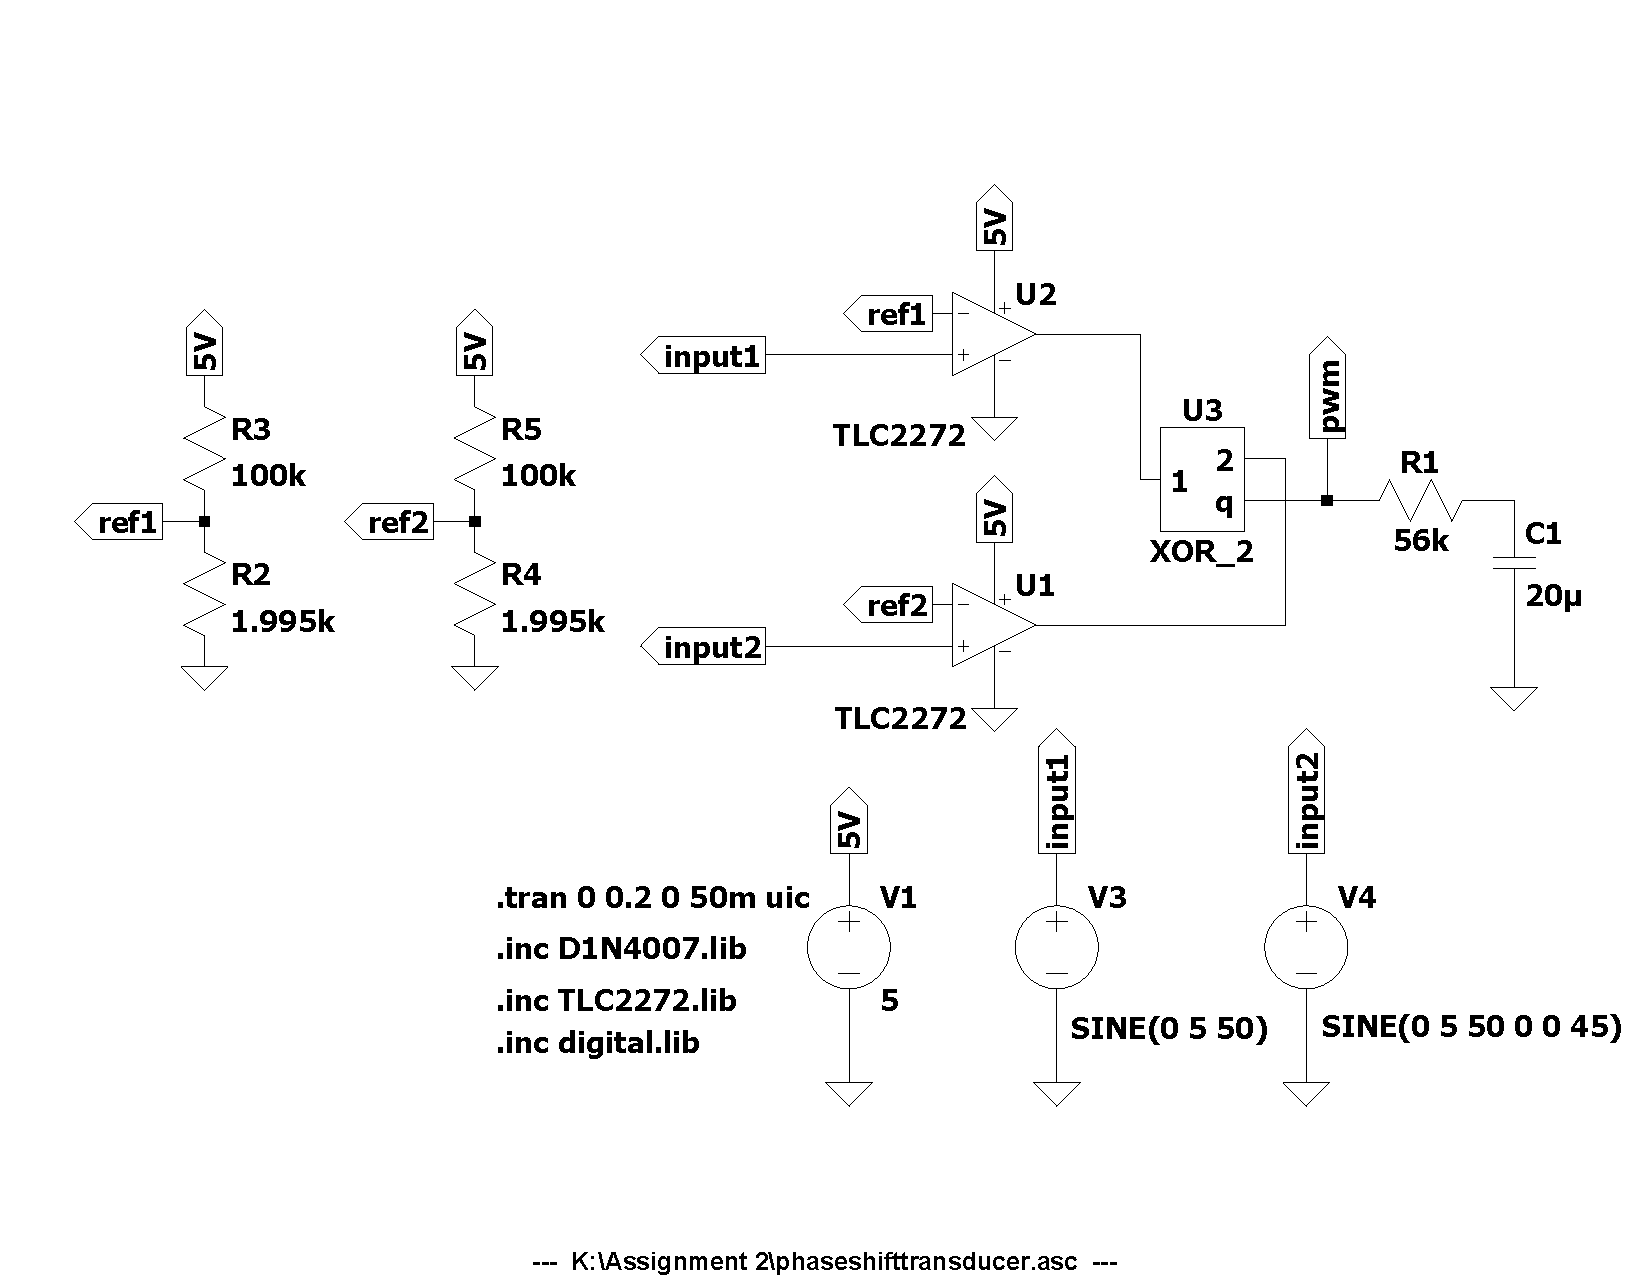
\includegraphics[width=0.5\linewidth]{./Figures/ptrans_circuit_diagram.pdf}
		    \caption{Phase-shift transducer circuit diagram.} \label{fig:ptrans_circuit_diagram}
 \end{figure}
 
\subsection{Design} \label{sec:phase_design}
The phase difference between the voltage and current signals was implemented by using an operational amplifier comparator as a zero crossing detector, in this configuration the input voltage was applied at the non inverting pin and the reference input was applied at the inverting input pin and was set to \SI{100}{\milli \volt} \cite{ZeroCrossingDetector} to ensure that noise would not interfere with the output of the comparator. These reference signals were implemented by using a voltage divider circuit, using Equation \ref{eq:voltagedivider} and by selecting $R_1$ as a $100k\Omega$ resistor a value for $R_2$ could be found as $1.995k\Omega$. These second resistors were implemented using a potentiometer so that the PWM output of the comparators could be calibrated under no load conditions as to provide a more accurate output. The operational amplifier used for this design was the TLC2272, this chip was chosen due to its rail to rail capabilities. Both of the comparators were used in single supply mode, thus its two saturated states corresponded to \SI{0}{\volt} and \SI{5}{\volt} respectively. \vspace{4mm} \newline
The input voltage to the zero crossing detector for the voltage level was taken as the output from the voltage divider network in Figure \ref{fig:vtrans_circuit_diagram}, labelled as $v_{meas}$, and the input voltage to the zero crossing detector for the current level was taken as the output from the gain stage in Figure \ref{fig:itrans_circuit_diagram}, labelled as $i_{meas}$. Both of these input signals had a maximum voltage of \SI{5}{\volt} and thus were within the limits of the differential mode input of the operational amplifiers. The phase delay between these two signals was found by using a XOR gate that would output a logical high for the duration that the two sinusoids were out of phase \cite{PWMref}. This XOR gate was implemented by using a CD4070B integrated chip, with this integrated circuit supplied by the \SI{5}{\volt} rail and ground respectively \cite{CD4070B:2003}. \vspace{4mm} \newline
%As the inputs of the XOR gate are periodic square wave signals, the output would be a square wave pulse train with varying duty cycle dependant on how out of phase the input signals are, thus the frequency domain equivalent of this circuit would be a series of dirac deltas at multiples of the fundamental frequency enveloped by sinc functions.
A crude low pass filter was implemented to convert the PWM signal to a DC output voltage \cite{PWMref}. The low pass filter was designed by using Equation \ref{eq:cutofffreqcap} and choosing a cut off frequency of 10Hz, where a fixed \SI{20}{\micro F} was selected and the resistor was implemented using a $\SI{56}{\kilo \Omega}$ potentiometer. This potentiometer was tuned until an output signal with an acceptable voltage ripple was obtained. As the output of this transducer had to be as accurate as possible all noise levels superimposed on the DC output voltage had to be kept to a minimum. This was achieved by implementing the smoothing capacitor at the output as two \SI{10}{\micro F} low ESR capacitors placed in parallel. Decoupling capacitors were also placed at the positive rails of the TLC2272 and the CD4070B to minimize the effects of the rail voltage noise on the output.
\begin{align}
    f_{cut-off}=\frac{1}{2\pi RC} 
   \label{eq:cutofffreqcap}
\end{align}
The transducer was designed to measure a phase angle difference of up to $180^o$, which corresponded to a DC output voltage of \SI{5}{\volt}, and as it was only necessary that the transducer had to measure phase angles with an accuracy of $1^o$ it was decided that an external gain stage was not necessary. %As the Arduino had a resolution of 4095 bits the input signal could be measured with an accuracy of up to \SI{4.888}{\milli V}, this was equal to an angle of $0.176^o$ per bit. 
Equation \ref{eq:angle_calc} was applied to convert the output DC voltage level to an angle in degrees, with Equation \ref{eq:angle_delta} demonstrating the effect of a small change in input phase angle on the DC output voltage, here it was that a 1mV noise measurement would produce an output measurement of $0.036^o$.

\begin{align}
    V_{meas} =\frac{\phi_{load}}{180^o} 5 \nonumber \\
    \phi_{load} =\frac{V_{meas}}{5} 180^o \label{eq:angle_calc} \\
    \delta \phi_{load} =\frac{\delta V_{meas}}{5} 180^o \label{eq:angle_delta}
\end{align}

\subsection{Simulation} \label{sec:ptrans_simu}
The phase transducer was tested in simulation by applying two out of phase signals at the input of the transducer and plotting the output DC voltage level. Given a load of 1k and $\SI{22}{\mu F}$ the output voltage was found to be 226mV, this is shown in Figure \ref{subfig:ptrans_simu_1k22u}. The transducer was also simulated with a load of 1k and $\SI{33}{\mu F}$, where the output voltage was found to be 151mV, this is shown in Figure \ref{subfig:ptrans_simu_1k33u}. From these figures and simulated measurements we can see that the transducer operated as expected.

\begin{figure}[!ht]
 \footnotesize
 \centering
    \begin{subfigure}[]{0.4\textwidth}
              \centering
  		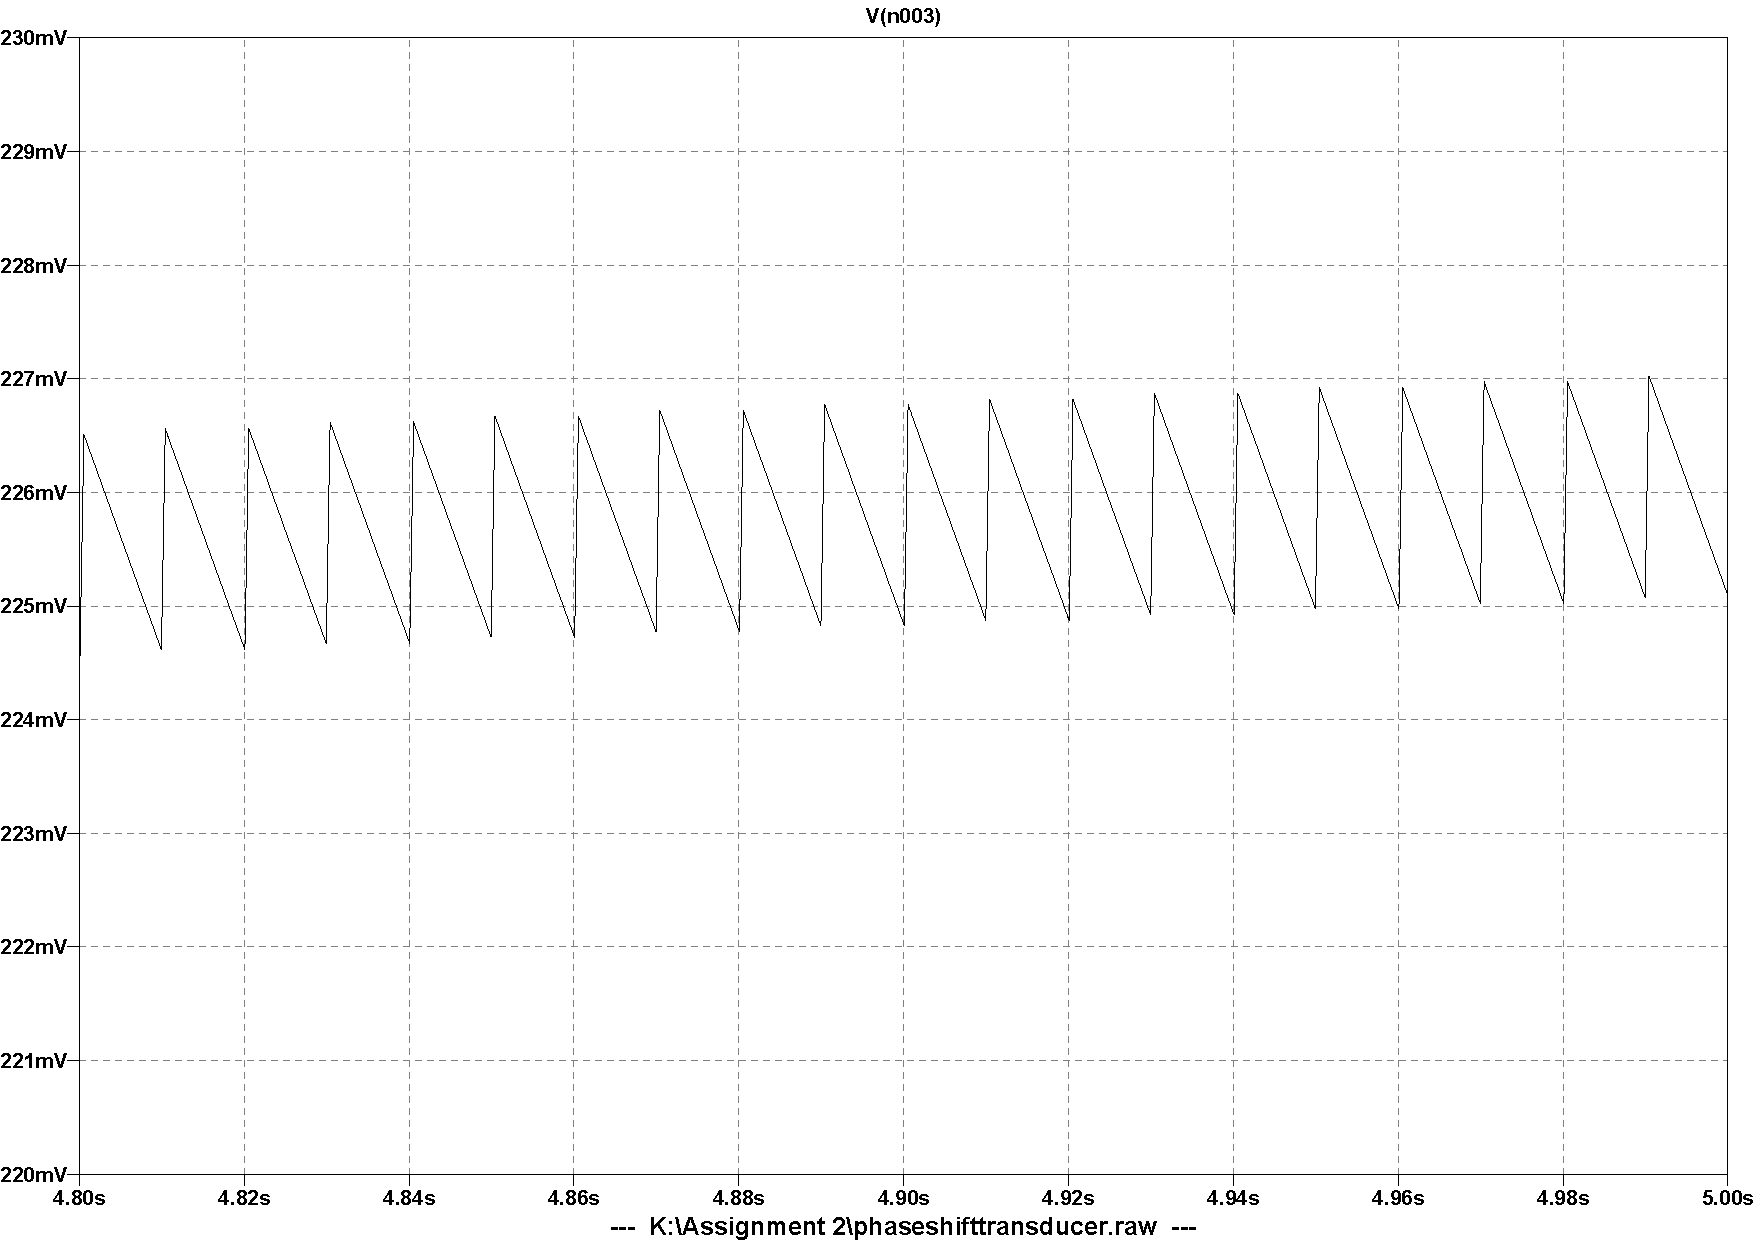
\includegraphics[width=1.0\linewidth]{./Figures/ptrans_simu_1k22u.pdf}
		    \caption{} \label{subfig:ptrans_simu_1k22u}
     \end{subfigure}
          \begin{subfigure}[]{0.4\textwidth}
             \centering
  		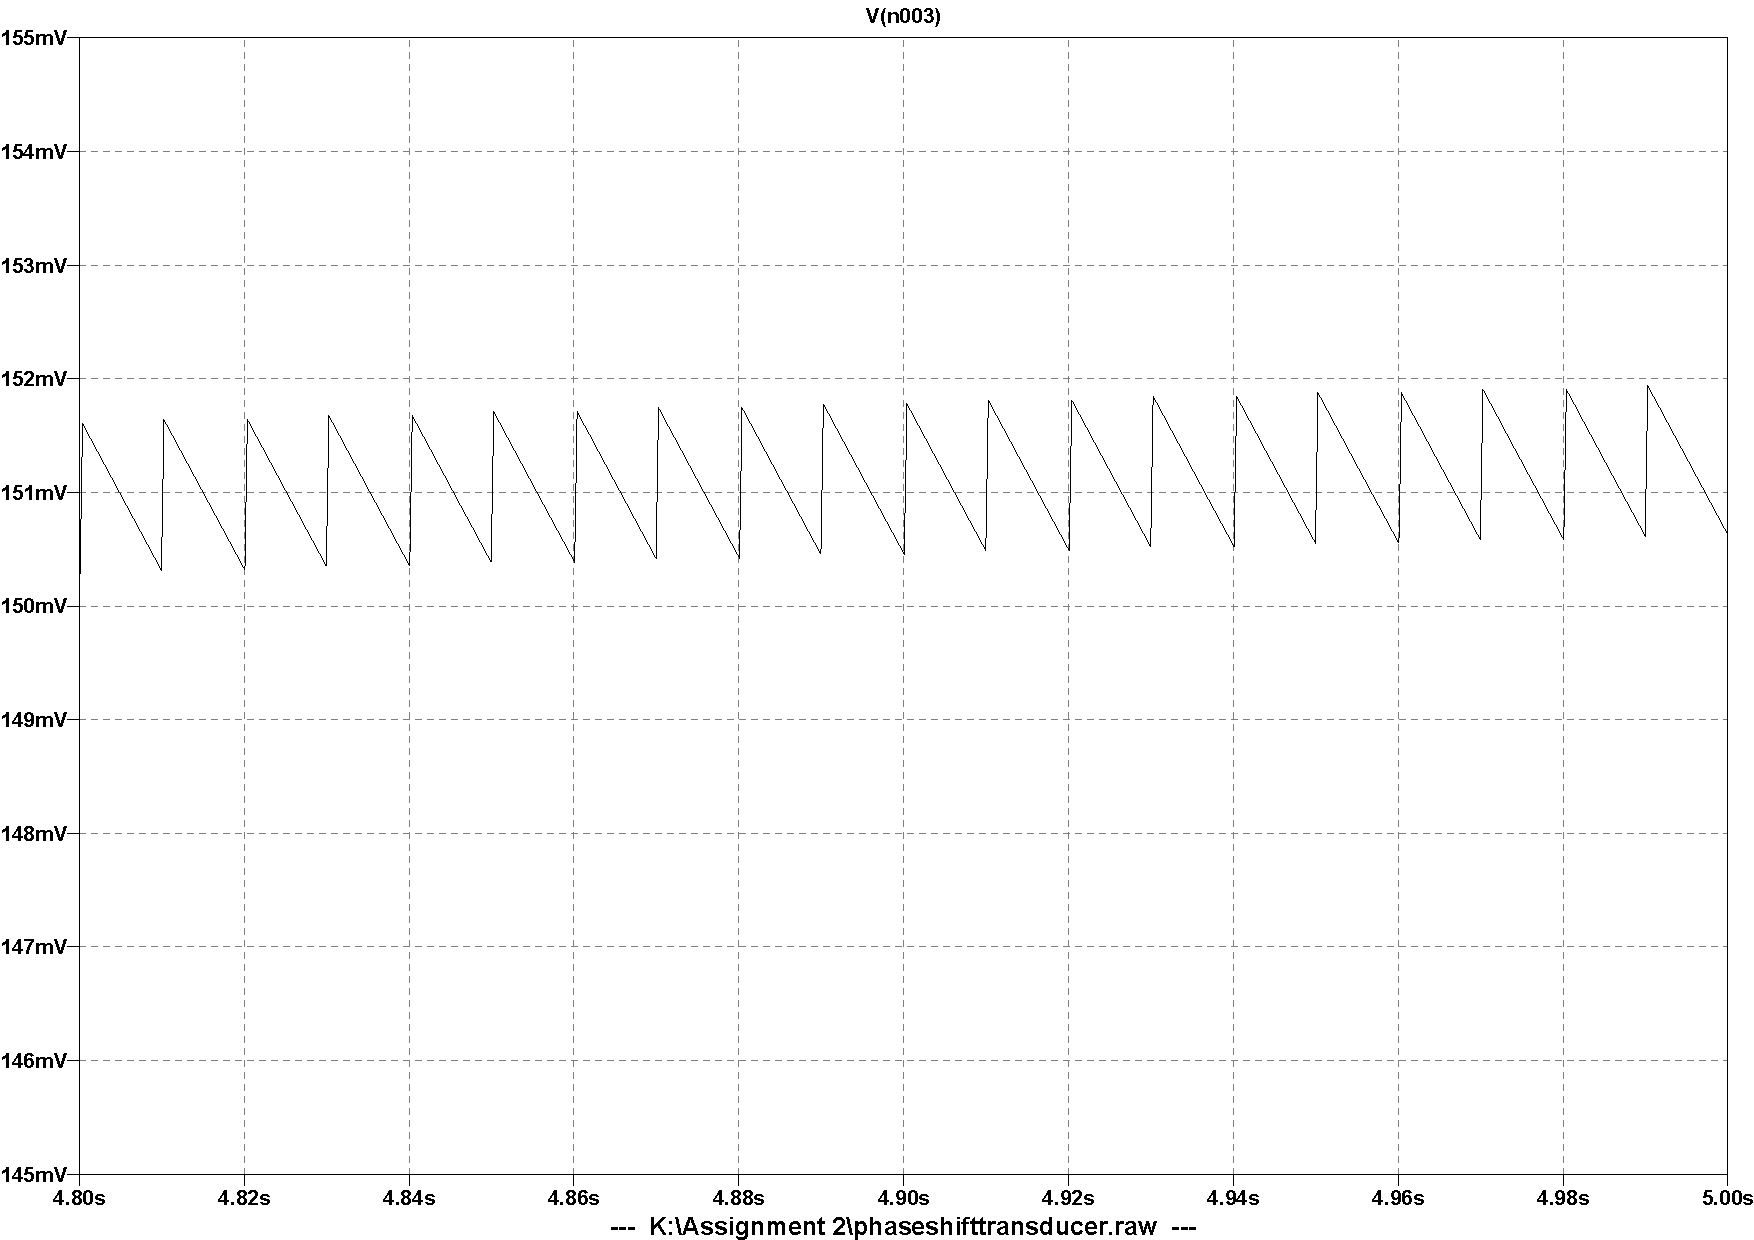
\includegraphics[width=1.0\linewidth]{./Figures/ptrans_simu_1k33u.pdf}
		   \caption{ } \label{subfig:ptrans_simu_1k33u}
     \end{subfigure}
    \begin{subfigure}[]{0.4\textwidth}
              \centering
  		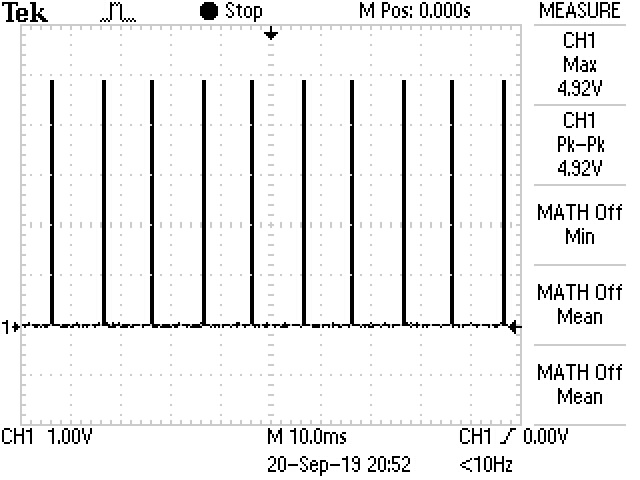
\includegraphics[width=1\linewidth]{./Figures/ptrans_meas_nom.JPG}
		    \caption{} \label{subfig:ptrans_meas_nom}
     \end{subfigure}
          \begin{subfigure}[]{0.4\textwidth}
             \centering
  		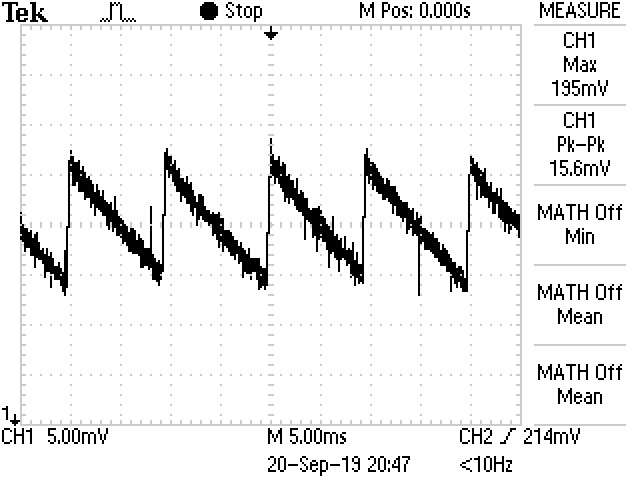
\includegraphics[width=1.0\linewidth]{./Figures/ptrans_meas_noise.JPG}
		   \caption{ } \label{subfig:ptrans_meas_noise}
     \end{subfigure}
     \caption[Phase shift transducer measurement results] {Phase-shift transducer results. (a) $1k\Omega$ 22uF reactive load output signal simulated. (b) $1k\Omega$ 33uF reactive load output signal simulated. (c) Mid-sized reactive load PWM signal measured. (d) Mid-sized reactive load measured DC output level and associated ripple. } \label{fig:ptrans_results}
\end{figure}

\subsection{Measurement} \label{sec:ptrans_meas}
To test whether the phase transducer worked in practice integrated tests were performed using various loads as inputs as to induce different phase changes. The results of these measurements are tabulated in Table \ref{tab:phasetransducerrealtests}. Here the measured shift column refers to the average time difference between the voltage and current signals crossing the zero axis, and the applied shift refers to this average time shift converted to a phase angle. \vspace{4mm} \newline 
The output DC voltage level was related to the input phase angle by Equation \ref{eq:angle_calc}, and given these measurements it was found that the largest angle deviation was found to differ by $0.96^o$, which was within the tolerance of $1^o$. Figure \ref{subfig:ptrans_meas_nom} shows the oscilloscope measurement of the output of the phase transducer as PWM signal given a mid range input of $1k\Omega$ and $\SI{22}{\mu F}$. After passing this PWM signal through a low pass filter a DC signal was obtained, the measured DC value and its associated ripple voltage is shown in Figure \ref{subfig:ptrans_meas_noise}. As with the other two transducers only the 5V rail was used and thus the main frequency component of the noise on the output was characterised by the 50Hz supply voltage frequency. Here it was found that the signal had a peak to peak voltage of only $\SI{15.6}{\milli V}$, and this result was less than the $\SI{27.78}{\milli V}$ accuracy required to ensure a measurement within $1^o$ of what was actually obtained. This confirms that the phase transducer fulfills all of the design requirements and was implemented successfully.

\section{Summary and implementation}
The signal conditioning circuitry implemented in this design met all of the design required and the practical circuit can be seen in Figure \ref{subfig:trans_pcb}. The voltage transducer design implemented in this system could detect input voltage peaks up to $\SI{34}{V}$ accurately within $\SI{150}{\milli V}$. The transducer successfully responded to a $\SI{1}{V}$ change in input within 1 second for voltage peaks above $\SI{18}{V}$. The current transducer design implemented could accurately detect currents up to $\SI{350}{\milli A}$ with an accuracy of less than $\SI{1}{\milli A}$, and could successfully react to a $\SI{10}{\milli A}$ change in input within 1 second. These aforementioned transducers were successfully implemented in the phase transducer design which could measure phase difference between the two input signals within an accuracy of $1^o$. All noise interference was successfully minimized in this design by the use of the low noise $\SI{5}{V}$ rail and the use of decoupling capacitors, further improving the quality of the design.

\begin{figure}[!ht]
    \centering
  		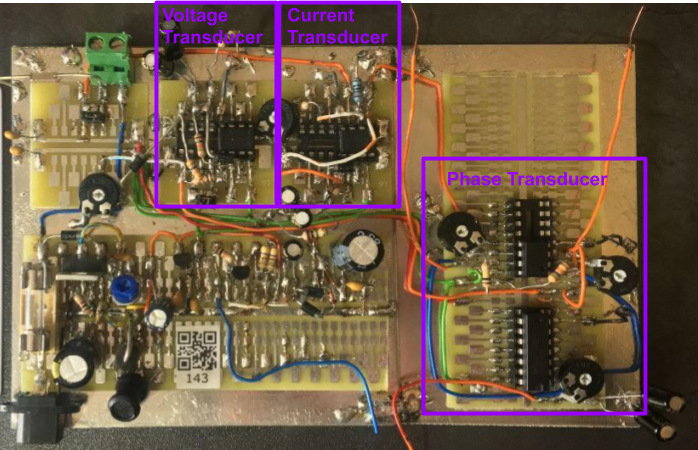
\includegraphics[width=0.55\linewidth]{./Figures/trans_pcb.png}
		   \caption{Implementation of the transducer circuitry. } \label{subfig:trans_pcb}
     \end{figure}



